\section{Auswertung}
\label{sec:Auswertung}
\subsection{Bestimmung der mittleren Reichweite}
Da der MCA nur Channel, keine konkreten Energien ausgibt, müssen diese über Dreisatz in Energien umgerechnet werden, wobei Channel 280 $\SI{4}{\mega \electronvolt}$ entspricht.
Aus dem in Abb.\ref{fig:Energie} mittels \eqref{eqn:gerade} gefitteten Ausgleich der ersten Messung erhält man die Parameter: $a_1 = \SI{-2.11 \pm 0.06}{\mega\eV}$, $b_1=\SI{4.06 \pm 0.03}{\mega\eV}$. Entsprechend liefert die zweite Messung $a_2 = \SI{-2.67 \pm 0.09}{\mega\eV}$, $b_2 = \SI{4.06 \pm 0.03}{\mega eV}$. Der Abstand der Sonde zum Zähler ist im ersten Durchlauf $x_1 = \SI{23}{\milli\meter}$, im zweiten $x_2 = \SI{29}{\milli\meter}$. Die Energiesteigung ergibt sich somit zu:

\begin{align*}
  -\frac{\symup{d}E_1}{\symup{d}x}=\SI{91.7 \pm 2.6}{\mega\eV\per\meter} \\
  -\frac{\symup{d}E_2}{\symup{d}x}=\SI{92.0 \pm 3.1}{\mega\eV\per\meter}.
\end{align*}

\begin{equation}
  f(x) = a\cdot x +b
  \label{eqn:gerade}
\end{equation}

\begin{figure}
  \centering
  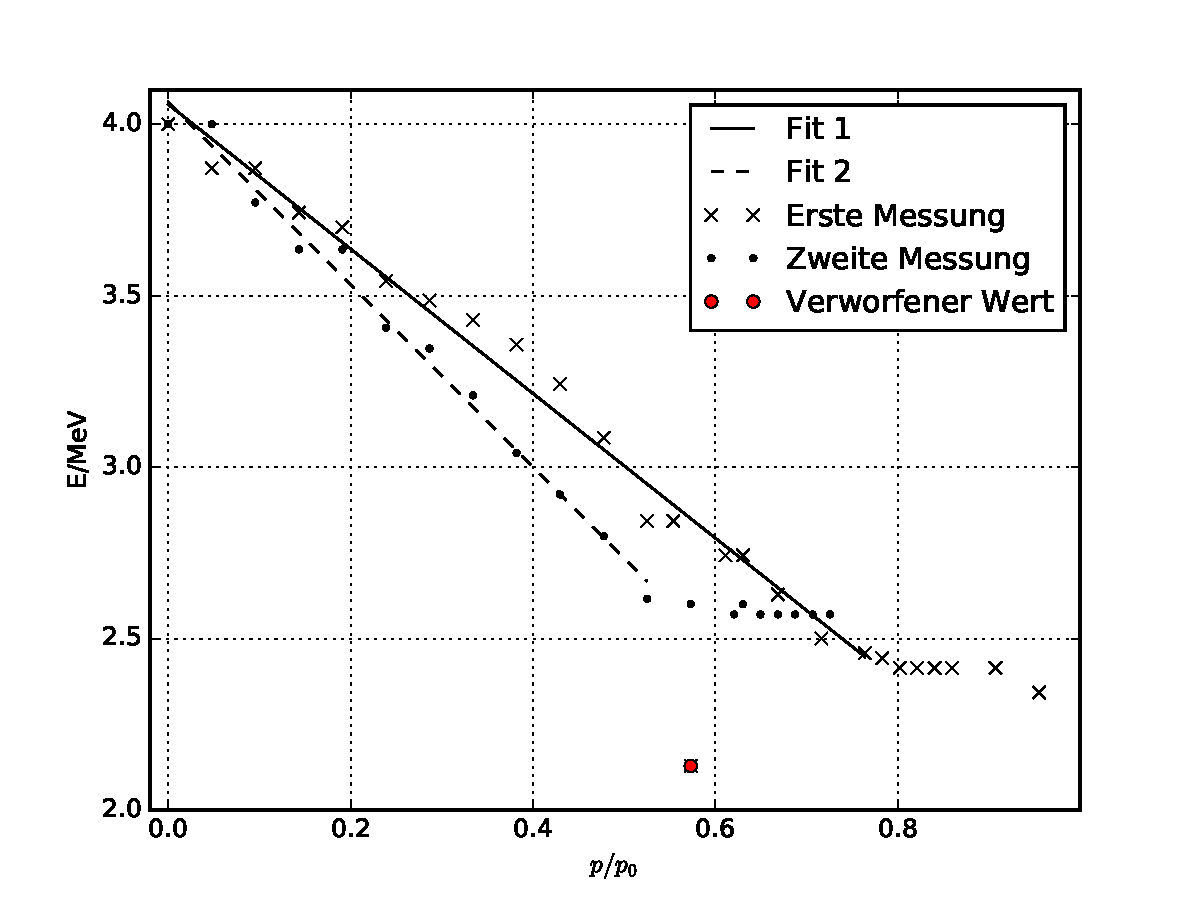
\includegraphics[height=7cm]{plots/Energie.pdf}
  \caption{Energie der gemessenen $\alpha$-Teilchen aufgetragen gegen den relativen Druck $p/p_0$}
  \label{fig:Energie}
\end{figure}

Für die Plateau-Phase erhält man eine gemittelte Zählrate von $f_1 = \SI{580\pm5}{\becquerel}$, bzw. $f_2 = \SI{377\pm9}{\becquerel}$. Wie Abb. \ref{fig:Rate} zu entnehmen, wurde für den Berreich des stärksten Abfalls ein linearer Fit gemäß \eqref{eqn:gerade} durchgeführt. Die Parameter hierfür sind:
\begin{align*}
  a_{f_1} &= -\SI{4163 \pm 925}{\becquerel} \\
  b_{f_1} &= \SI{3580 \pm 743}{\becquerel} \\
  a_{f_2} &= -\SI{1235 \pm 45}{\becquerel} \\
  b_{f_2} &= \SI{872 \pm 28}{\becquerel}
\end{align*}
Mit diesen Geraden kann man die Mittlere Reichweite der Strahlung durch Umstellung nach dem effektiven Weg und einsetzen von $f_{1/2}$ bzw. $f_{2/2}$ berechnen zu:

\begin{align*}
  R_1 &= \frac{x_o}{a_{f_1}}\left(f_1/2-b_{f_1}\right)=\SI{0.018 \pm 0.006}{\meter} \\
  R_2 &= \SI{0.016 \pm 0.001}{\meter}
\end{align*}

Diese Fehler ergeben sich durch

\begin{align*}
  \Delta R &= \sqrt{\left(\frac{\delta}{\delta a}\frac{x_o}{a_{f}}\left(f/2-b_{f}\right)\right)^2 \cdot \Delta a^2 + \left(\frac{\delta}{\delta b}\frac{x_o}{a_{f}}\left(f/2-b_{f}\right)\right)^2 \cdot \Delta b^2} \\
  &= \sqrt{\left(\frac{x_o}{a_{f}^2}\left(f/2-b_{f}\right)\right)^2 \cdot \Delta a^2 + \left(\frac{x_o}{a_{f}}\right)^2 \cdot \Delta b^2}
\end{align*}


\begin{figure}
  \centering
  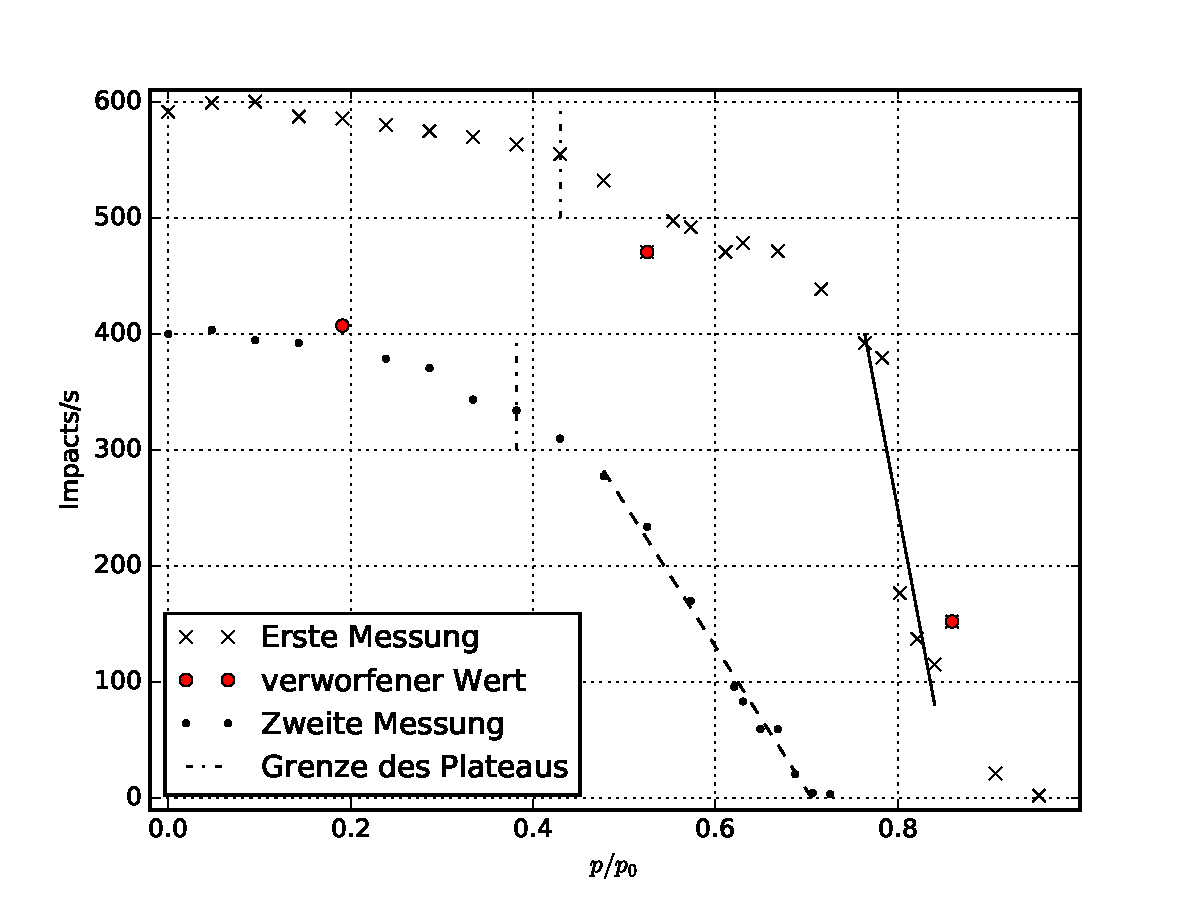
\includegraphics[height=7cm]{plots/Rate.pdf}
  \caption{Zählrate aufgetragen gegen den relativen Druck $p/p_0$}
  \label{fig:Rate}
\end{figure}

\subsection{Statistik des Zerfalls}
Die genommenen Messwerte wurden als normiertes Histogram (d.h. alle Balken addiert ergeben 1) in Abb. \ref{fig:hist} dargestellt, d.h. das Histogram wurde so normiert, dass die Summe über alle Balken 1 beträgt. Die eingezeichnete Fit-Kurve stellt eine Gauß-Normalverteilung gemäß
\begin{equation}
  G(x) = \frac{A}{\sigma\cdot\sqrt(2\pi)}e^{-0.5 \left(\frac{x-m}{\sigma}\right)^2}
  \label{eqn:gauß}
\end{equation}
dar. Hierbei ist  $\sigma=\SI{19.81 \pm 1.07}{\becquerel}$ die Standardabweichung und $m= \SI{533.98}{\becquerel}$ der Mittelwert der aufgenommenen Werte. Im Histogram sind 10 Balken aufgelöst, was einer Breite von ca. $\SI{10}{\becquerel}$ entspricht und somit höher auflösend gewählt ist als die Standardabweichung.

 \begin{figure}
   \centering
   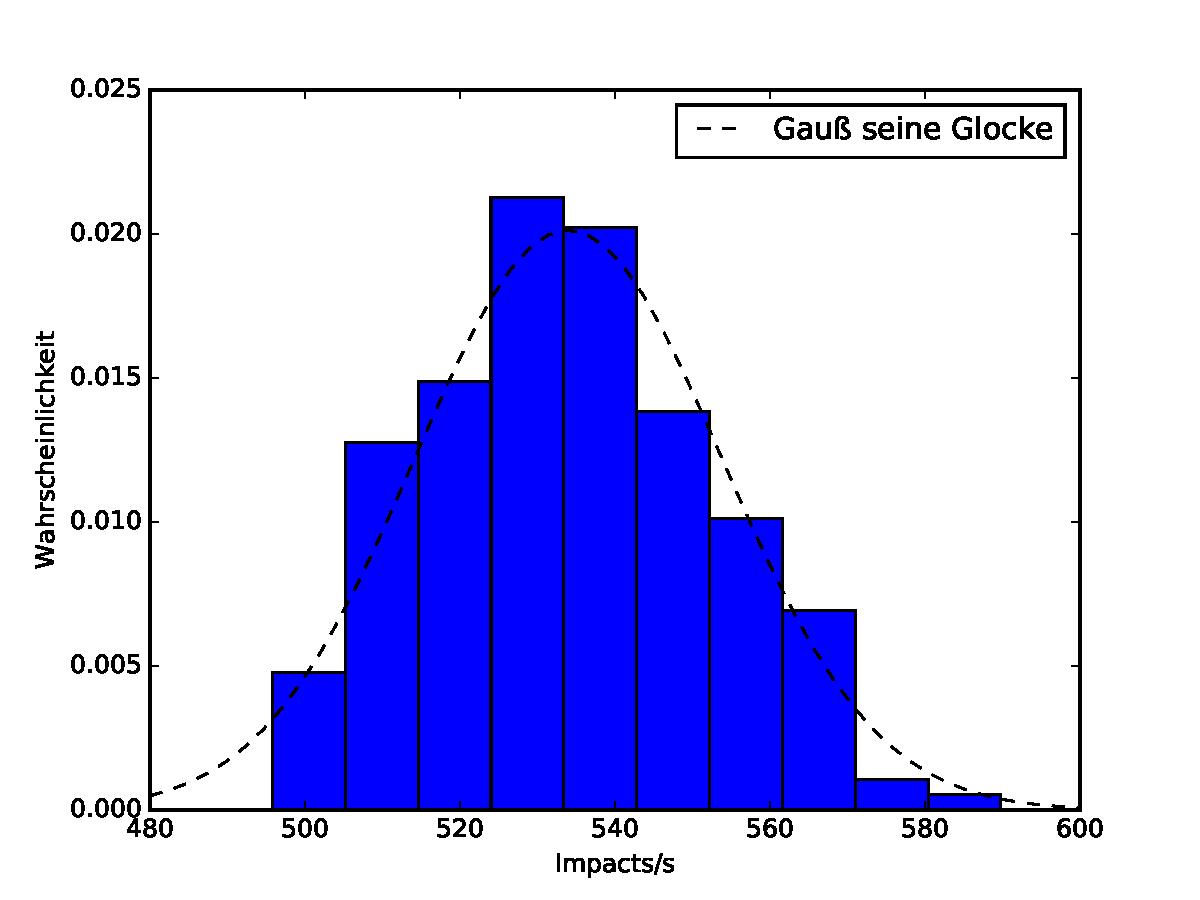
\includegraphics[height=7cm]{plots/Statistik.pdf}
   \caption{Histogram zur Zählrate}
   \label{fig:hist}
 \end{figure}
